\documentclass{article}
\usepackage[a4paper, total={6.5in, 9in}]{geometry}
\usepackage{amsmath}
\usepackage{graphicx}

\title{Computational Methods: Problem Set 5}
\author{Ian O'Donnell}
\date{\vspace{-5ex}}
\begin{document}
\maketitle

\section*{Simulation}
\begin{center}
    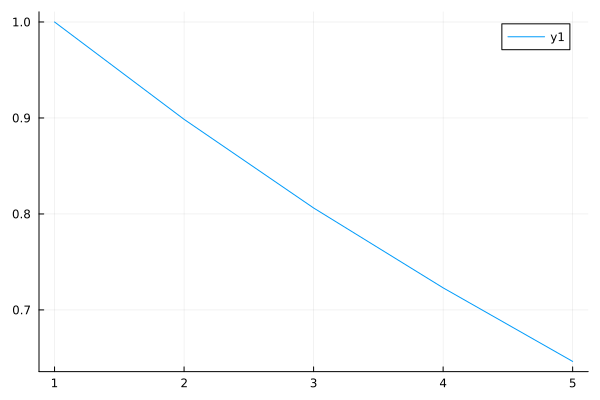
\includegraphics[scale = 0.6]{p1.png} \\
    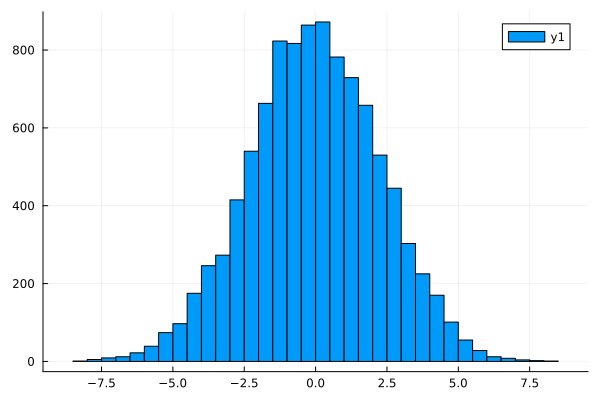
\includegraphics[scale = 0.6]{p6.png}
\end{center}
    


\section*{Tauchen}
\begin{center}
    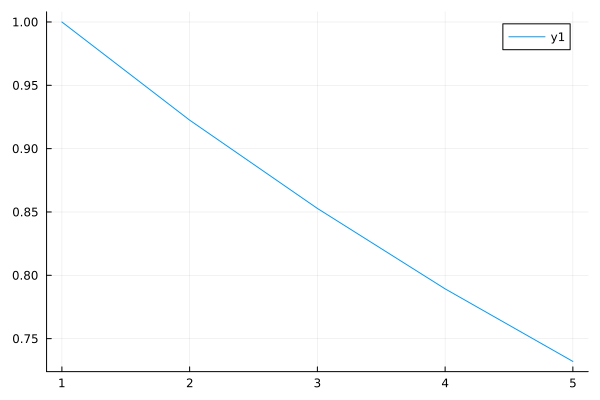
\includegraphics[scale = 0.6]{p2.png} \\
    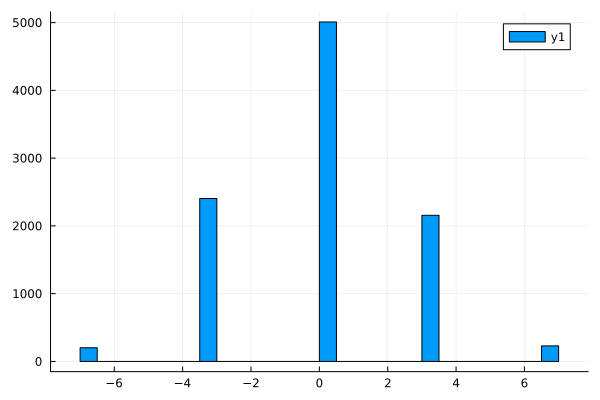
\includegraphics[scale = 0.6]{p7.png} \\

    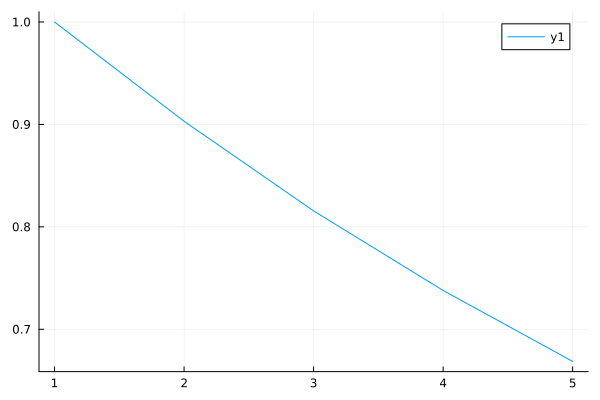
\includegraphics[scale = 0.6]{p3.png} \\
    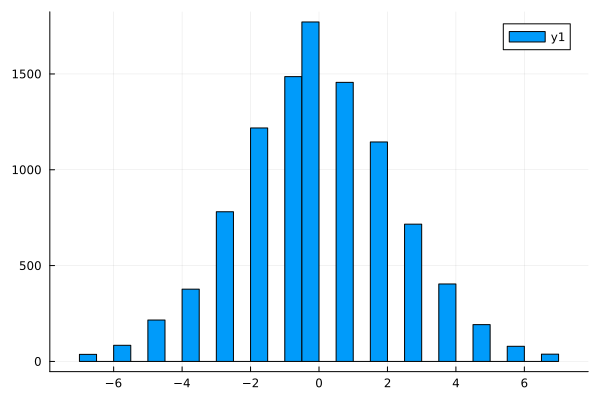
\includegraphics[scale = 0.6]{p8.png} \\

    

\end{center}


\section*{Rouwenhorst}
\begin{center}
    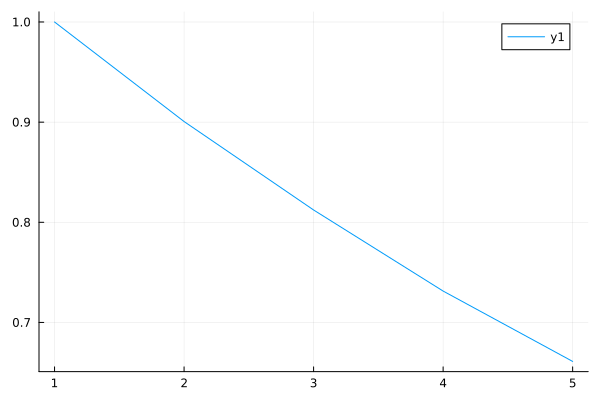
\includegraphics[scale = 0.6]{p4.png} \\
    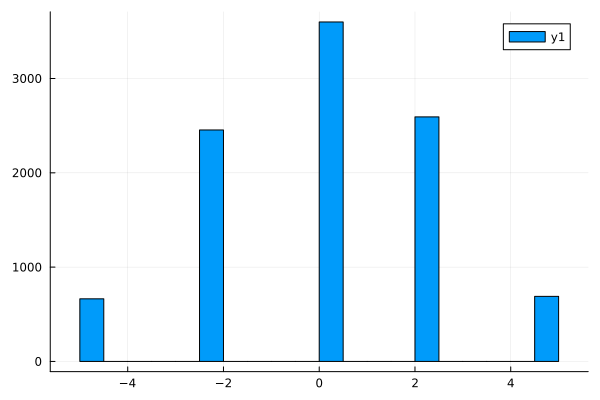
\includegraphics[scale = 0.6]{p9.png} \\
    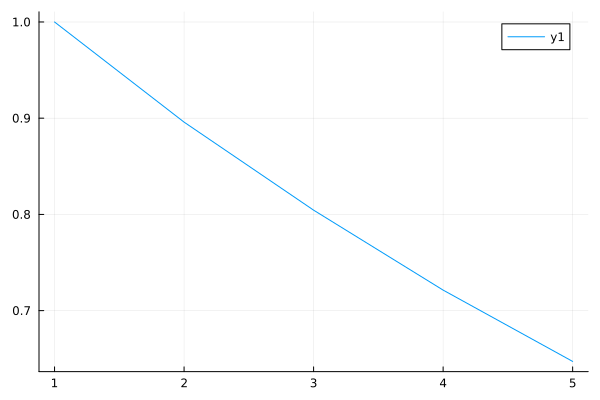
\includegraphics[scale = 0.6]{p5.png} \\
    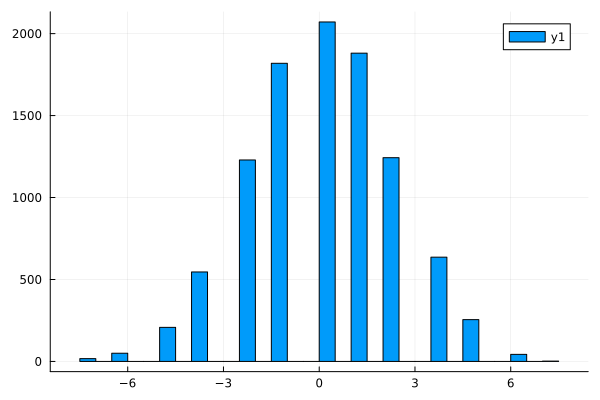
\includegraphics[scale = 0.6]{p11.png} \\
\end{center}

\section*{Value Function Iteration}

\begin{center}
    \includegraphics*[scale = 0.6]{p7b.png}
    \includegraphics*[scale = 0.6]{p8b.png}
    \includegraphics*[scale = 0.6]{p9b.png}
\end{center}

\end{document}